%% This is file `jcomp-template.tex',
%% 
%% Copyright 2017 Elsevier Ltd
%% 
%% This file is part of the 'Elsarticle Bundle'.
%% ---------------------------------------------
%% 
%% It may be distributed under the conditions of the LaTeX Project Public
%% License, either version 1.2 of this license or (at your option) any
%% later version.  The latest version of this license is in
%%    http://www.latex-project.org/lppl.txt
%% and version 1.2 or later is part of all distributions of LaTeX
%% version 1999/12/01 or later.
%% 
%% The list of all files belonging to the 'Elsarticle Bundle' is
%% given in the file `manifest.txt'.
%% 
%% Template article for Elsevier's document class `elsarticle'
%% with harvard style bibliographic references
%%
%% $Id: jcomp-template.tex 100 2017-07-14 13:15:12Z rishi $
%%
%% Use the option review to obtain double line spacing
%\documentclass[times,review,preprint,authoryear]{elsarticle}

%% Use the options `twocolumn,final' to obtain the final layout
%% Use longtitle option to break abstract to multiple pages if overfull.
%% For Review pdf (With double line spacing)
\documentclass[times,twocolumn,final]{elsarticle}
%% For abstracts longer than one page.
%\documentclass[times,twocolumn,review,longtitle]{elsarticle}
%% For Review pdf without preprint line
%\documentclass[times,twocolumn,review,nopreprintline]{elsarticle}
%% Final pdf
%\documentclass[times,final]{elsarticle}
%%
%\documentclass[times,twocolumn,final,longtitle]{elsarticle}
%%


%% Stylefile to load JCOMP template
\usepackage{jcomp}
\usepackage{framed,multirow}
\usepackage{amsmath}
%% The amssymb package provides various useful mathematical symbols
\usepackage{amssymb}
\usepackage{latexsym}

% Following three lines are needed for this document.
% If you are not loading colors or url, then these are
% not required.
\usepackage{url}
\usepackage{xcolor}
\definecolor{newcolor}{rgb}{.8,.349,.1}

\journal{Computer Methods and Programs in Biomedicine}

\begin{document}

\verso{Anahita A. Seresti \textit{et al}}

\begin{frontmatter}

\title{Non-Invasive Estimation of Coronary Velocity: A Computational Framework for Computed Tomography Perfusion Imaging \tnoteref{tnote1}}%


\author[1]{Anahita \snm{A. Seresti}}

\author[2]{M. Owais \snm{Khan}\corref{cor1}}
\cortext[cor1]{Corresponding author: Department of Electrical, Computer and Biomedical Engineering, Toronto Metropolitan University, Toronto, 350 Victoria Street, Toronto, Ontario, M5B 2K3, Canada; Email: owaiskhan@torontomu.ca }


\address[1]{Department of Electrical, Computer and Biomedical Engineering, Toronto Metropolitan University, 350 Victoria Street, Toronto, M5B 0A1, Canada}


\received{1 May 2013}
\finalform{10 May 2013}
\accepted{13 May 2013}
\availableonline{15 May 2013}
%\communicated{S. Sarkar}


\begin{abstract}
%%%
    
\textbf{Background and Objectives}: Ischemic heart disease (IHD) results from insufficient blood flow to the myocardium, primarily caused by coronary artery stenosis. Existing clinical methods rely on invasive procedures for assessing coronary hemodynamics. Computational methods, particularly those based on coronary CT angiography (cCTA) and CT myocardial perfusion imaging (CT-MPI), offer non-invasive alternatives.

\textbf{Methods}: This study introduces a computational framework leveraging CT-MPI for estimating blood velocity in stenosed coronary arteries under steady flow conditions. The framework integrates diverse simulation techniques, including computational fluid dynamics (CFD) and advection-diffusion simulations. 

\textbf{Results}: Results demonstrate promising agreement between estimated and assigned velocities, suggesting the potential of this method for non-invasive coronary flow assessment. The observed dependence on Reynolds number highlights the need for further refinement and investigation into estimation methods.

\textbf{Conclusions}: Future work may involve exploring advanced models to mitigate biases and enhance accuracy. Ultimately, this research contributes to the potential of non-invasive assessment of blood flow dynamics from routine scans, with implications for improved diagnosis and targeted therapeutic interventions.
%%%%
\end{abstract}


\begin{keyword}
% MSC codes here, in the form: \MSC code \sep code
% or \MSC[2008] code \sep code (2000 is the default)
% Keywords
\KWD Coronary Artery Imaging \sep CT Myocardial Perfusion Imaging \sep Computational Fluid Dynamics \sep Blood Velocity Estimation \sep Non-Invasive Coronary Flow Assessment
\end{keyword}


\end{frontmatter}

%\linenumbers

%% main text

%--------------------------------------- Introduction -----------------------------------------

\section{Introduction}
Ischemic heart disease (IHD) arises from inadequate blood flow to the myocardium, primarily due to coronary artery stenosis. While coronary artery anatomy plays a crucial role in understanding blood perfusion, it often fails to directly correlate with the pathophysiology of stenosis causing flow restriction. Consequently, the current clinical standard for assessing the physiological effects of coronary disease on hemodynamics relies on invasive pressure catheterization during angiography. However, the lack of a routine non-invasive flow assessment remains a significant challenge, hindering our understanding of the underlying mechanisms of coronary flow limitations \cite{al2018percutaneous, toth2013fractional}.

Computational methods based on coronary CT angiography (cCTA) offer a promising avenue for capturing hemodynamic features of the blood flow in coronary arteries. By leveraging cCTA-derived coronary geometry, computational fluid dynamics (CFD) simulations enable comprehensive assessments of hemodynamics, including pressure, velocity, and wall shear stress \cite{assen2020computed,papamanolis2021myocardial,bove2003computational,he2022medical,khan2021low}. However, the accuracy of these assessments hinges on accurate boundary conditions and flow split assumptions \cite{kung2011vitro,cook2017diagnostic}.

Another potentially valuable CT-based technique for visualizing and quantifying coronary blood flow is CT myocardial perfusion imaging (CT-MPI). Although unexplored for this purpose, the dynamic transit of contrast through the coronary arteries holds promise for calculating mean blood velocity. In 2015, Eslami [1] pioneered the transluminal attenuation flow encoding (TAFE) method, utilizing experimental phantom CT images to estimate blood velocity from contrast transition along a tapered vessel. Assuming unidirectional flow and dominant convective forces, TAFE calculates mean flow rate. Eslami subsequently introduced a CFD-based correction factor to further refine accuracy [2]. While their studies focused on experimental data under laminar flow conditions, we have demonstrated the potential of this approach under a wider range of flow conditions, suggesting its applicability to CT-MPI-based applications.

In this study, we present a computational framework for estimating blood velocity in stenosed coronary arteries with steady flow based on contrast agent transition. Our pipeline encompasses diverse simulation techniques to model blood flow, contrast agent transit, and velocity calculation. Following a detailed description of the theoretical background and simulation setup, we validate our method by comparing calculated velocities with pre-assigned values under steady flow conditions. Finally, we conclude by discussing the implications and potential future directions of this work.

%--------------------------------------- METHODOLOGY -----------------------------------------
\section{Methods}

%------------- Problem Statement ----------------------
\subsection{Contrast Transport and Blood Flow}
To rigorously validate the accuracy and robustness of our velocity estimation pipeline, we established a multi-step computational framework simulating both blood flow and contrast agent dispersion within a stenosed arterial segment. This framework encompassed two key components:
%Figure 0
\begin{figure*}[!t]
    \centering
    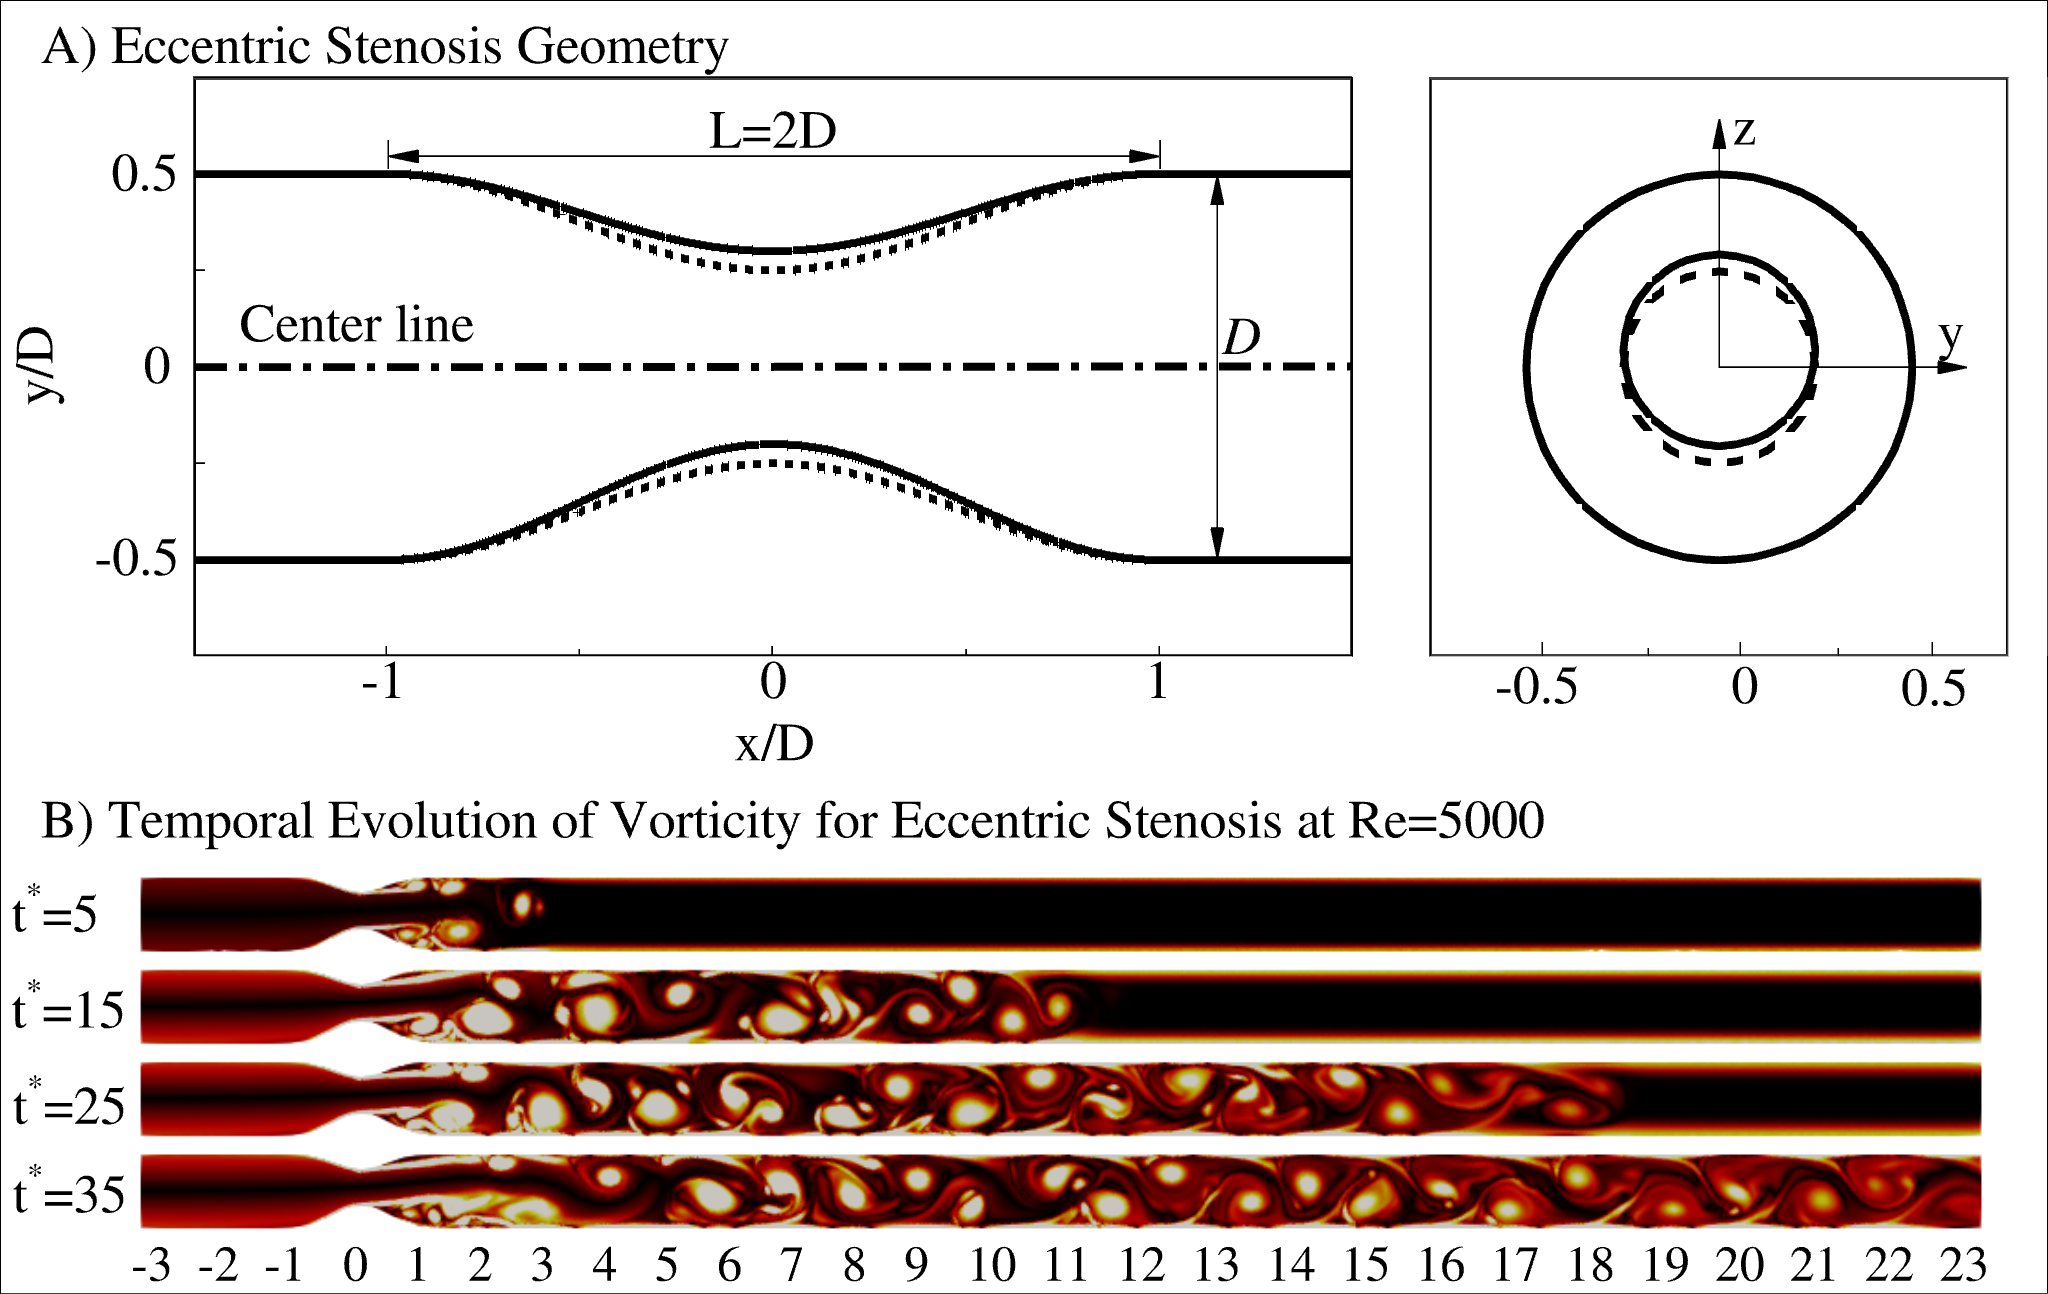
\includegraphics[width=0.95\textwidth]{./Figures/Figure1_StenosisModel.png}
    \caption{Eccentric Stenosis Geometry}
    \label{Figure:stenosed_geometry}
    \end{figure*}
\begin{enumerate}
    \item \textit{Stenosed Vessel Geometry}: This study employed a three-dimensional, idealized model of a non-axisymmetric stenosis to represent the complex geometric variations observed in diverse vasculatures. The modeled artery extended along the x-axis from -9 cm to 72 cm, with the stenosis located at x = 0 causing a 75\% reduction in the cross-sectional area. Notably, the stenosis throat incorporated an eccentricity to promote flow instability without requiring additional velocity field perturbations. The specific geometry is depicted in Figure ~\ref{Figure:stenosed_geometry}. This configuration was inspired by a prior study investigating turbulent flow transition in stenosed arteries [reference].
    \item \textit{Modeling blood flow in stenosed arteries}: In order to implement our pipeline of flow and contrast transition in the stenosed artery, two partial differential equations are the key components: Navier-Stokes equations, simulating the blood flow assuming a newtonian and incompressible fluid [], and Advection-Diffusion equation, modeling the contrast agent transport in the blood []. The governing equations of the Navier-Stokes equation is presented below:
        \begin{equation}
            \dfrac{\partial U}{\partial t} + (U. \nabla)U + \dfrac{\nabla P}{\rho} = \nu \nabla^2U,\quad \quad \quad \nabla.U=0
        \end{equation}
        Where $U$ is the time-dependent velocity vector field, $P$ is the pressure field inside the geometry domain, $\rho$ is the blood flow density, and $\nu$ is the dynamic viscosity. A Neumann type boundary condition was assigned to the inlet of the vessel and a non-slip boundary condition ($u=0$) was assigned to the walls. To encompass the range of flow regimes encountered in diverse arterial beds, we varied the Reynolds number (Re) from 100 to 1000 in increments of 100. This parameter selection captures the spectrum of physiological flow conditions observed in coronaries and cerebral arteries (Re ~ 100-300), carotid arteries (Re ~ 400-600), and the aorta (Re ~ 700-1000). By simulating across this extensive Re range, our investigation encompasses the complex, multi-regime flow dynamics found in human vasculature. 
    \item \textit{Modeling contrast agent transition in coronaries}: The next crucial step in our framework involves simulating the spatiotemporal evolution of the contrast agent concentration within the vasculature. This necessitates incorporating the complex interplay between advection, driven by the bulk blood flow, and diffusion, arising from microscopic Brownian motion. To adequately capture this interplay, we employ the advection-diffusion equation, a fundamental partial differential equation widely used in fluid dynamics and mass transport phenomena. In our context, the advection-diffusion equation takes the following form, where $C(x,y,z;t)(\frac{ml}{mg})$ represents the contrast agent concentration at spatial location $(x,y,z)$ and time t:
        \begin{equation}
            \dfrac{\partial C}{\partial t} + (U.\nabla )C = D\nabla ^2C
        \end{equation}
        Here, $U(x,y,z)$ denotes the blood velocity at the spatial location $(x,y,z)$, which derives the transport of contrast agent in the blood and is determined by the preceding CFD simulation. D is the diffusion coefficient, which quantifies the rate of contrast spread due to random molecular motion, with a value of 0.04 cm²/s as reported by []. To assign the inlet boundary conditions of the contrast agent we used the following equation []:
        \begin{equation}
            C_{inlet} = C_{min} + 0.5(C_{max}-C_{min})[1-cos({\pi}\frac{t-T_s}{T_d})],
        \end{equation}
        where $C_{min}$ and $C_{max}$ are the minimum and maximum values of the contrast in the inlet of the artery, chosen to be 0 and 1 respectively. And $T_s$ is the time at which the bolus arrives and $T_d$ is time for which the advection-diffusion is considered.
    \item \textit{Contrast Dispersion}: Following the simulations, we extract mean velocity information from the observed contrast transition. Based on the simulated contrast bolus, we perform an inverse estimation to compute the centerline velocity along the arterial segment. While solving the full contrast dispersion equation would be ideal, the inherent limitations of CT-MPI in terms of spatial resolution and noise hinder the accurate reconstruction of the 3D velocity field, particularly in the context of coronary arteries. Therefore, to account for these limitations, we adopted a simplified approach assuming unidirectional flow with negligible radial dispersion of contrast. This allowed us to estimate the average velocity across the arterial lumen, albeit sacrificing the full spatiotemporal resolution offered by the advection-diffusion equation:
        \begin{equation}
            v_{mean} = \dfrac{\frac{\partial C}{\partial t}}{-\frac{\partial C}{\partial x}}
        \end{equation}
        This equation relates the centerline velocity ($V$) at a specific axial location ($x$) along the artery to the temporal and spatial variations in contrast concentration ($C$) observed during the simulation. The numerator, representing the rate of change in contrast over time ($\frac{\partial C}{\partial t}$), is obtained by computing the instantaneous derivative of the time-intensity curve at the desired location. Likewise, the denominator, reflecting the spatial gradient of contrast along the centerline ($\frac{\partial C}{\partial x}$), is calculated by taking the derivative of the contrast profile with respect to the axial coordinate at the peak contrast intensity.

\end{enumerate}

%---------------- Simulations Setup ------------------------
\subsection{Simulations Setup}
%FIGURE 1
\begin{figure*}[!t]
    \centering
    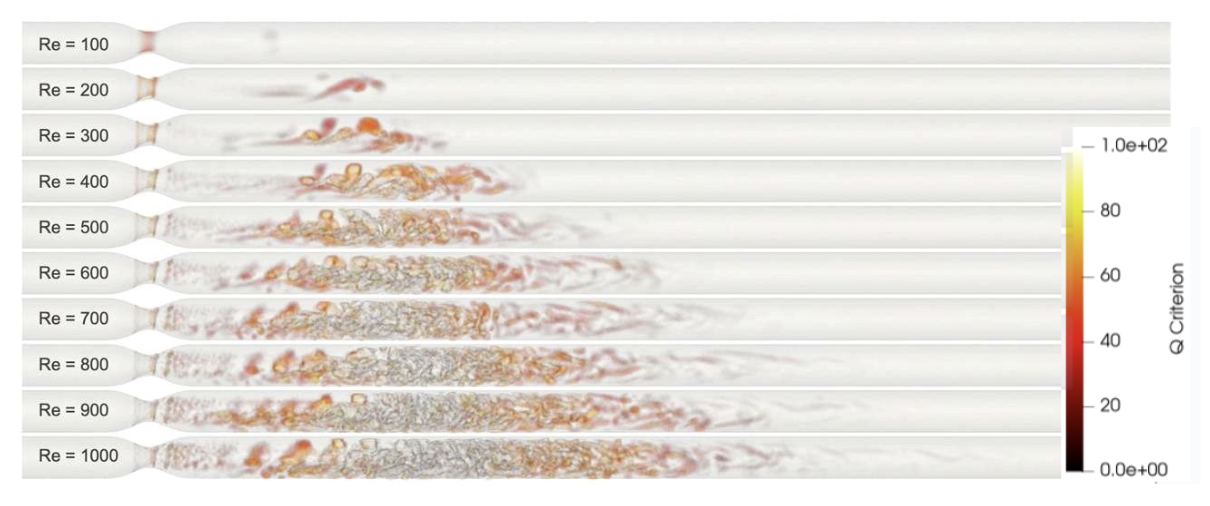
\includegraphics[width=0.8\textwidth]{./Figures/Figure2_results_CFD.png}
    \caption{The results of implementing CFD simulations in stenosed pipe. changing $Re=100-1000$}
    \label{fig:Results_CFD}
    
    \end{figure*}
\textit{CFD simulations} To characterize the onset and nature of turbulence transition in a stenosed artery, we employed direct numerical simulations (DNS) of the steady flow within a non-axisymmetric 3D stenosis model (Khan et al., 2018). Using the Oasis flow solver, we implemented CFD simulations of the Navier-Stokes equations for incompressible Newtonian blood ($\mu = 0.004 Pa*s$, $\rho = 1057 \frac{kg}{m^{3}}$). To accurately capture the evolving turbulent features, time steps were meticulously chosen as $0.0001$ seconds. A pulsatile Womersley profile was applied at the inlet to mimic realistic blood flow, while the outlet boundary conditions were dynamically adjusted through a pressure coupling scheme. The Navier-Stokes equations were solved for blood pressure and velocity using a second-order polynomial interpolation for velocity and a first-order scheme for pressure. The resulting velocity fields were subsequently exported for further analysis in the Advection-Diffusion simulation stage. This DNS approach was repeated across a range of Reynolds numbers ($Re = 100-1000$). The stenosed artery geometry was meshed with approximately 6000 triangular elements. The simulations were done on Niagara supercomputers of the Canada Research Alliance [].
\textit{Advection Diffusion Simulations} To model the transport of a contrast agent within the fluid flow, we employed the FEniCS framework [reference] to numerically solve the advection-diffusion equation. The velocity field, computed a priori using CFD simulations, was incorporated as the convection velocity within the advection term of the governing equation. The FEniCS framework facilitated the solution of the variational form of the equation using finite element methods. For each time step, the corresponding CFD velocity field was loaded to ensure consistency with the evolving flow dynamics. Inlet boundary conditions were prescribed in accordance with equation #, with $C_{min} = 0$, $C_{max} = 1$, $T_s = 0$, and $T_d$ adjusted between 12 and 85 seconds to accommodate the range of Reynolds numbers investigated. The spatiotemporal evolution of contrast agent concentration along the vessel is visualized in Figure ~\ref{Figure:contast_transition}.
\textit{Contrast Dispersion Simulations} To quantify the mean velocity within the vessel, we employed a back-calculation procedure based on the advection-diffusion equation (Equation #). This process involved two key steps:
\begin{enumerate}
    \item \textit{Extraction of Attenuation Curves} We first extracted the contrast agent's attenuation over time at the inlet of the vessel from the advection-diffusion simulation results, forming the time-attenuation curve. Additionally, we extracted the attenuation profile along the vessel's centerline at the peak time of contrast agent concentration, creating the centerline-attenuation curve.
    \item \textit{Linear Regression Modeling and Mean Velocity Calculation} Each extracted curve was then subjected to linear regression analysis, establishing a linear relationship between attenuation and the respective independent variable (time for the time-attenuation curve and spatial position for the centerline-attenuation curve). The slopes of the fitted linear models, representing the temporal and spatial concentration gradients ($\frac{\partial C}{\partial t}$ and $\frac{\partial C}{\partial x}$, respectively), were subsequently incorporated into equation # to back-calculate the mean velocity within the vessel.
\end{enumerate}
This approach enabled us to leverage the simulated advection-diffusion data to quantify the flow velocity without requiring direct measurement, providing valuable insights into the fluid dynamics within the vessel.

%------------------------------------ RESULTS ------------------------------------------------
\section{Results}
In our framework, multiple simulations were conducted to derive meaningful insights. The obtained results are summarized as follows:
\subsection{CFD Simulations}
Figure~\ref{Figure:Results_CFD} illustrates the Q-criterion, providing a visual representation of turbulent transition along the artery at various Reynolds numbers ($Re = 100-1000$). The CFD simulations aimed to assign a steady velocity to the stenotic pipe, ranging from 1.33 cm/s to 13.3 cm/s at different Reynolds numbers.
%Figure 2
\begin{figure*}[!t]
    \centering
    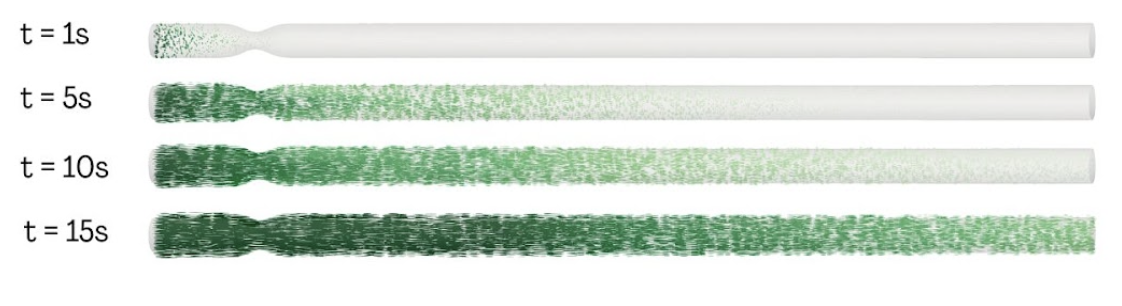
\includegraphics[width=0.95\textwidth]{./Figures/Figure3_results_advection_diffusion.png}
    \caption{Advection Diffusion Simulation Results, Contrast transition as the result of convection-diffusion simulations for $Re=1000$ in after 1, 5, 10 and 15 sec of running the simulations.}
    \label{Figure:Results_AdvDiff}
    \end{figure*}
\subsection{Advection-Diffusion Simulation}
The advection-diffusion setup was adjusted and validated against theoretical formulations. Figure~\ref{Figure:Results_AdvDiff} depicts the contrast dynamics at $Re = 1000$ at four time points ($t = 1, 5, 10, 15$ seconds), showcasing contrast perfusion along the artery. The final output illustrates the motion of contrast agents driven by the assigned velocity.
\subsection{Contrast Dispersion Simulation}
Results of the contrast dispersion, estimating velocity, were compared to the mean velocity assigned in the CFD simulations and summarized in Table~\ref{Table:Results_ContrastDisp}. The mean velocity error ranged from 0.1\% to 9\%, with an average of 2.5\% for different Reynolds numbers. The transit delay varied from 46\% to 65\% of the simulation run-time. An observed increase in the transit delay to simulation run-time ratio was noted with higher Reynolds numbers. The correlation coefficient for calculated velocity vs. Reynold's number.
\begin{table}[h]
    \centering
    \caption{Comparison of the CFD assigned velocity and the estimated velocity using our contrast dispersion method at varying Reynolds numbers and Advection-Diffusion simulation run-times.}
    \label{Table:VelocityComparison}
    \begin{tabular}{ccccccccccc}
    \hline
    \multicolumn{1}{c}{Re} & \multicolumn{1}{c}{run-time (s)} & \multicolumn{1}{c}{$V_{CFD}$} & \multicolumn{1}{c}{$V_{est}$} & \multicolumn{1}{c}{Err (\%)} \\
    \hline
    100   & 85   & 1.3    & 1.20   & 9.22 \\
    200   & 45   & 2.6    & 2.52   & 5.06 \\
    300   & 30   & 3.9    & 3.63   & 9.05 \\
    400   & 25   & 5.3    & 4.83   & 9.25 \\
    500   & 18   & 6.6    & 6.50   & 2.38 \\
    600   & 16   & 7.9    & 7.75   & 3.01 \\
    700   & 15   & 9.3    & 9.04   & 3.05 \\
    800   & 14   & 10.6   & 10.46  & 1.86 \\
    900   & 13   & 11.9   & 11.88  & 0.90 \\
    1000  & 12   & 13.3   & 13.31  & 0.12 \\
    \hline
    \end{tabular}
    \end{table}

%2D Non-axisymmetric Stenosis
%\subsection{Test Case B: 2D Non-Axisymmetric Stenosis at Re=5000}
%Figure ~\ref{fig:Results_2}A show the cross-section velocity distribution for the $sine$, $tanh$ and $swish$ activation functions with increasing number of sensor points. The $sine$ activation function was able to capture the oscillations in the flow field even with only 200 sensor points, while at least 400 points were needed to reconstruct the oscillatory flow patterns in the post-stenotic regions for $tanh$ and $swish$ activation functions. These observations are also evident from the quantitative analysis in Figure ~\ref{fig:Results_2}C, which shows that $sine$ activation function was able to converge to an error of approximately 25\% with a sensor point density of only 16 (i.e., 400 sensor points), while both $tanh$ and $swish$ activation functions needed a sensor point density of approximately 40 (i.e, 1000 sensor point) to converge to the same error levels. In addition, only $sine$ activation function showed a monotonic reduction in errors while both $tanh$ and $swish$ activation functions demonstrated a non-monotonic reduction in errors. 



%Figure 4
%\begin{figure*}[!t]
%\centering
%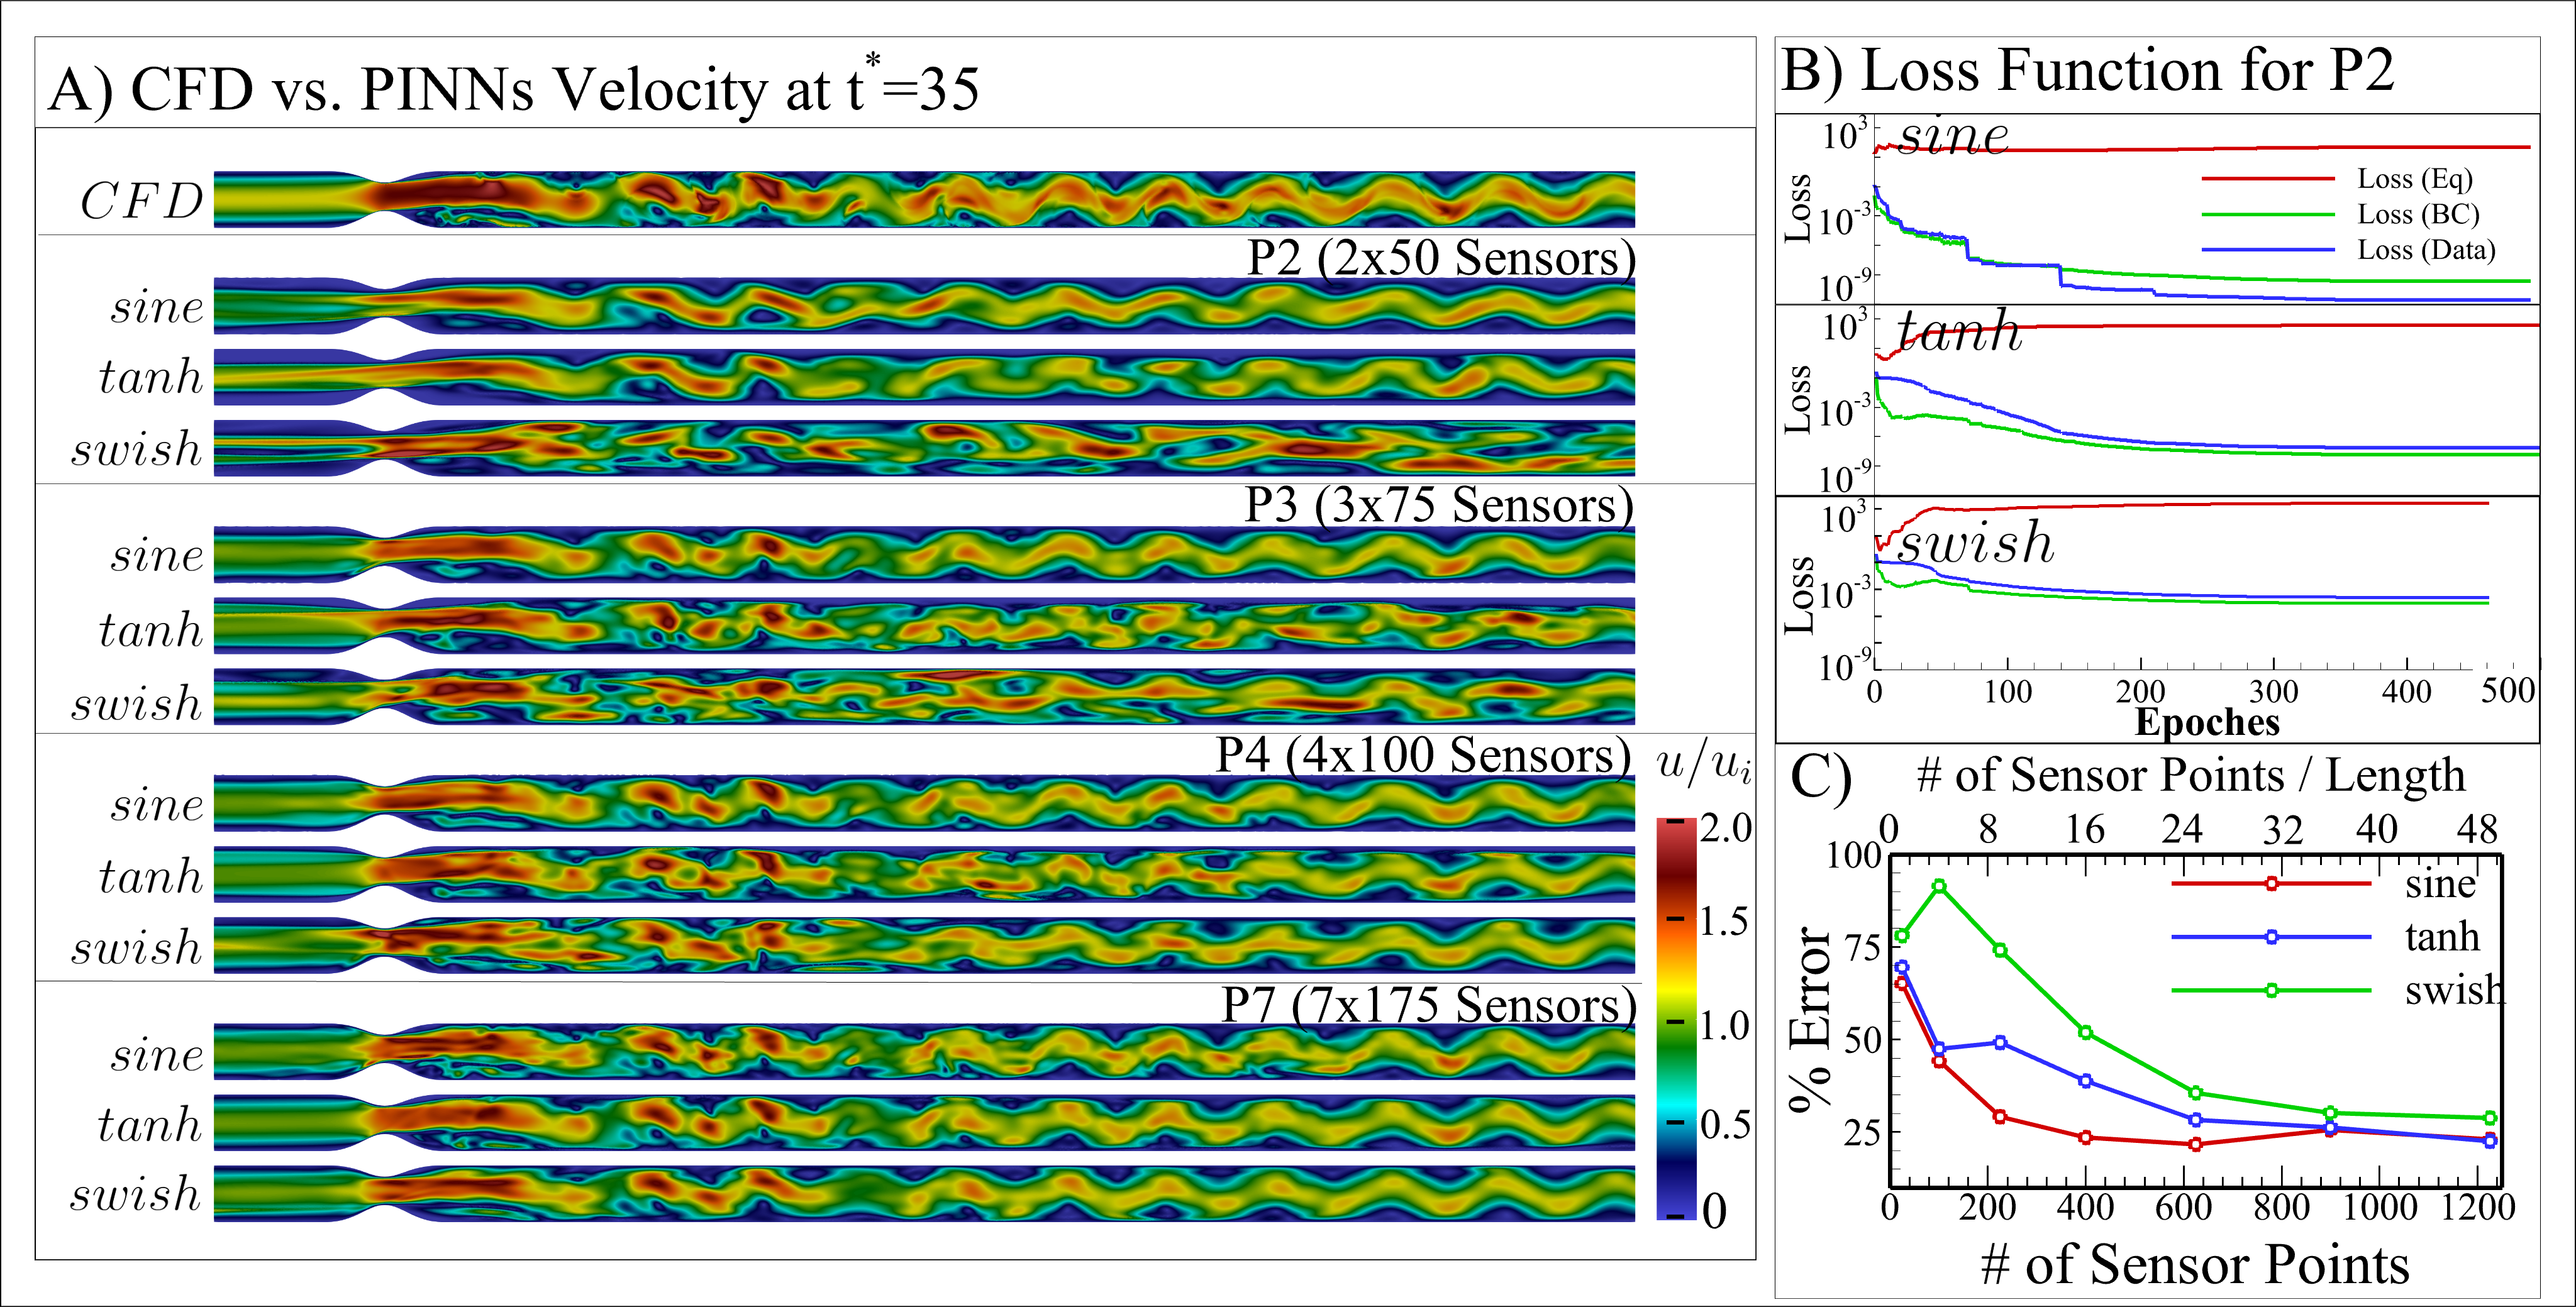
\includegraphics[width=0.95\textwidth]{./Figures/Figure4_StenosisResults_v2}
%\caption{PINNs solution for $sine$, $swish$ and $tanh$ activation functions for the 2D non-axisymmetric stenosis model at non-dimensional time of $t^{*}=35$ and Reynolds number of 5000. A) Reconstructed stream-wise velocity maps with increasing number of sensor points; B) Loss functions for P2 (i.e., with 2x5 sensors); C) Percent errors for the three activation functions with increasing sensor points and sensor point density.}
%\label{fig:Results_2}
%\end{figure*}


%3D Aortic Geometry
%\subsection{Test Case C: Patient-Specific 3D Aortic Geometry}
%Figure ~\ref{fig:Results_5} shows the performance of $sine$, $tanh$, and $swish$ activation functions in a 3D patient-specific aortic geometry at peak systole. Based on the qualitative velocity maps shown in Figure ~\ref{fig:Results_5}, it can be noted that a sensor point density of 40 (i.e, 800 sensor points) was needed to reconstruct the gross flow patterns observed in the ground-truth CFD simulations. The quantitative analysis, shown in Figure ~\ref{fig:Results_5}C, demonstrates that both $sine$ and $tanh$ had similar errors, while $swish$ had comparatively higher errors for the same number of sensor data points.

%POD analysis was performed to visualize the eigenspectra of the velocity field reconstructed from the three activation functions. Figure ~\ref{fig:Results_6} shows that for the case with 200 sensor points, all three activation functions showed similar Eigen spectra. However, with increasing number of sensor points, the $sine$ activation function was able to capture the energy content at higher modes much better than the other two activation functions, highlighting its ability to obtain high-frequency spatial structures in the velocity field . For example, for case with 800 sensor points and above, both $tanh$ and $swish$ activation functions were unable to adequately capture the kinetic energy in modes greater than 10. On the other hand, $sine$ activation function was able to better capture the energy content at these modes, matching well to the Eigen spectra obtained from the ground-truth CFD simulations. 

%Figure 5
%\begin{figure*}[!t]
%\centering
%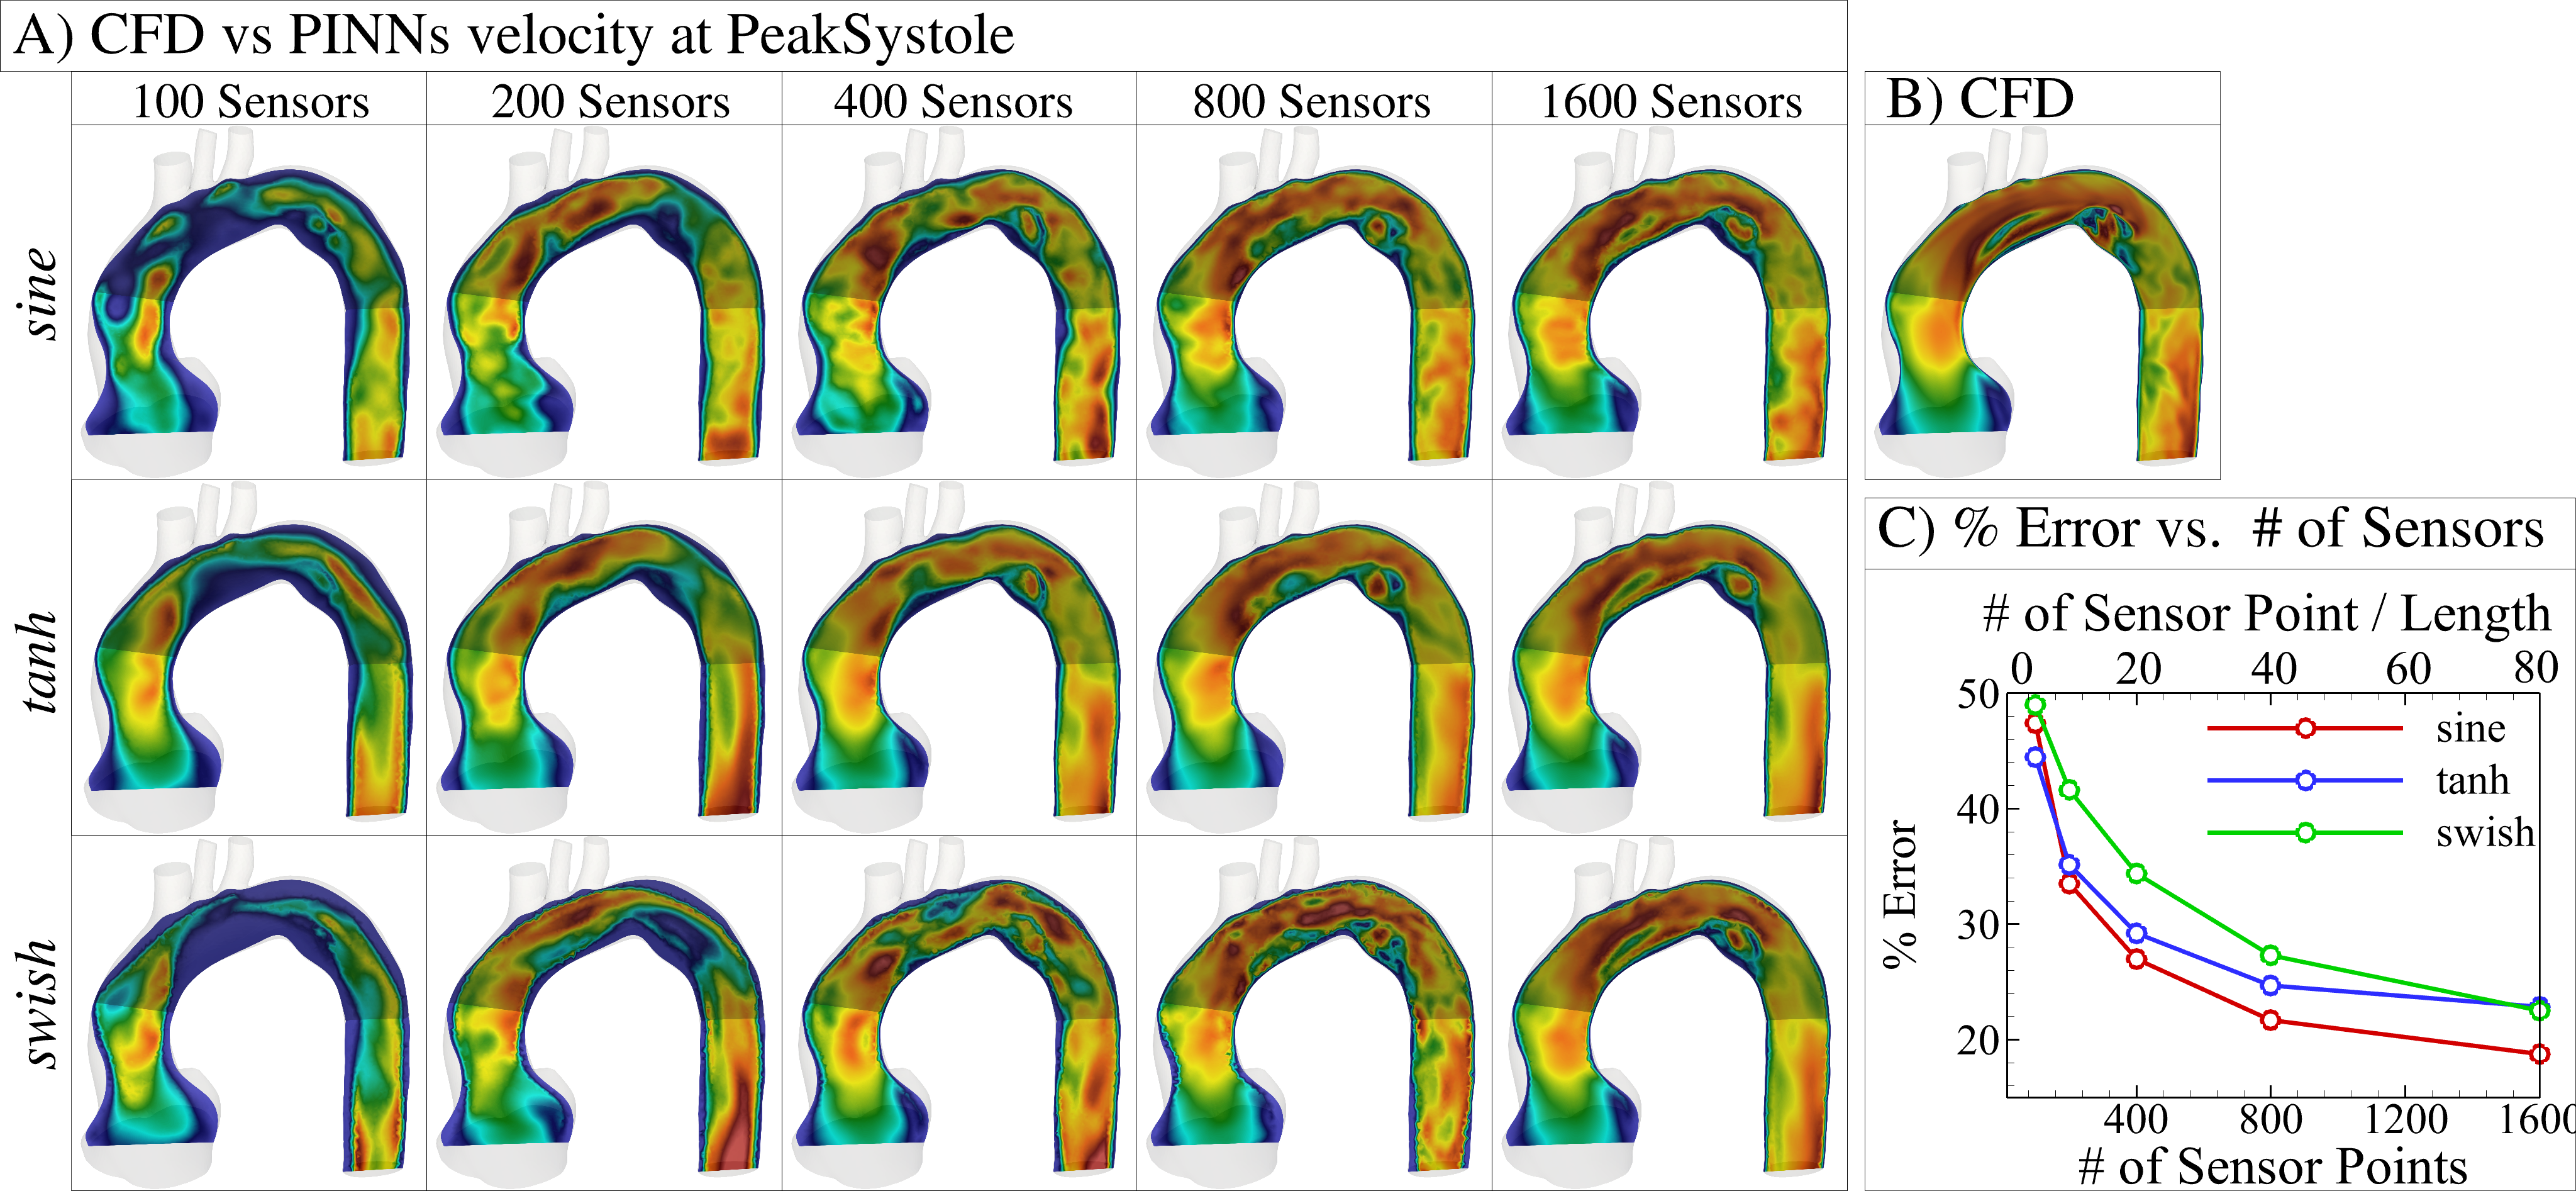
\includegraphics[width=0.95\textwidth]{./Figures/Figure5_Aorta}
%\caption{PINN solution for $sine$, $swish$ and $tanh$ activation functions for the 3D patient-specific aortic model at peak systole and Reynolds number of 823. A) PINNs-derived velocity maps with increasing number of sensor points from $100-1600$ at peak systole; B) Ground-truth solution obtained from CFD simulations; C)  Percent errors for the three activation functions with increasing sensor points and sensor point density. }
%\label{fig:Results_5}
%\end{figure*}

%Figure 6
%\begin{figure*}[!t]
%\centering
%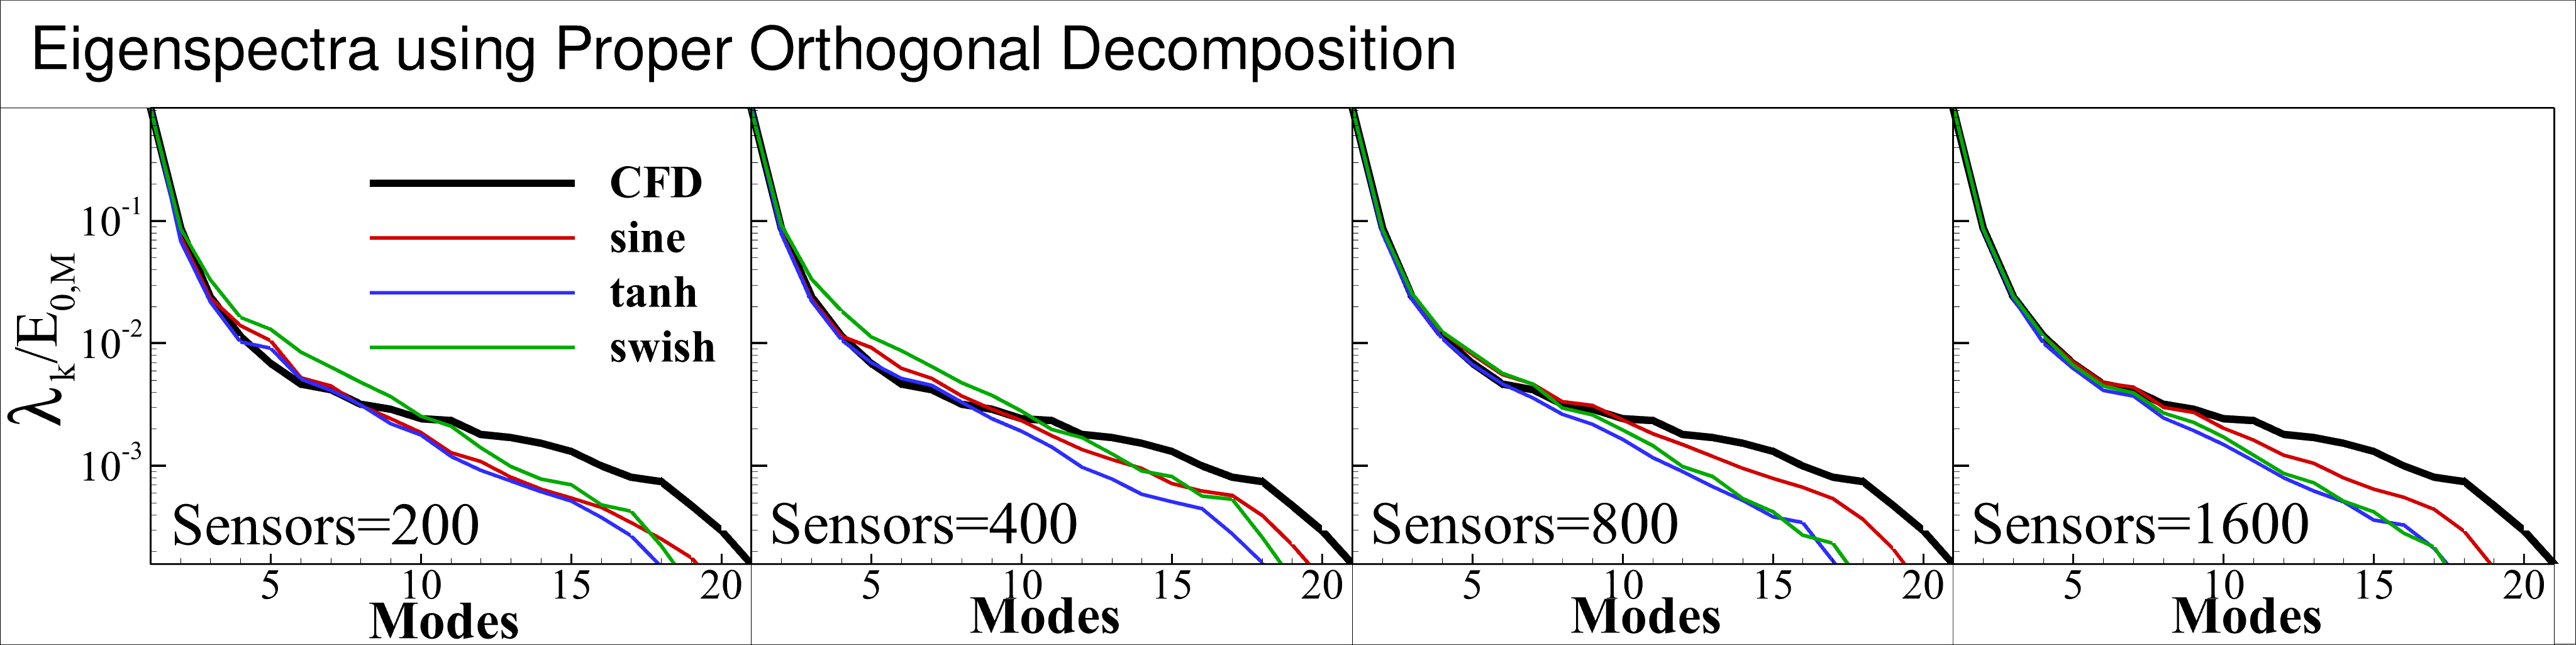
\includegraphics[width=0.95\textwidth]{./Figures/Figure6_Aorta_POD}
%\caption{Eigenspectra of temporal autocorrelation derived from proper orthogonal decomposition analysis for the 3D aorta model. Eigenvalue for each mode has been normalized by the sum of all eigenvalues from modes 0 to 20.}
%\label{fig:Results_6}
%\end{figure*}

%%%%%%%%%%%%%%%%% DISCUSSION %%%%%%%%%%%%%%%%%%%%
\section{Discussion}

Our findings underscore the potential of estimating lumen velocity through contrast perfusion imaging, despite inherent errors influenced by the flow regime. Notably, the estimated velocities closely align with the assigned velocities in CFD simulations across the Reynolds number spectrum, with errors predominantly below 10\%. Importantly, higher Reynolds numbers correspond to shorter simulation run-times and smaller percentage errors. In aggregate, the data suggests robust agreement between estimated and assigned velocities, indicating the efficacy of our method across diverse flow conditions.

These results bear significant implications for the expanding domain of non-invasive coronary flow assessment employing CT-MPI. The observed correlation between accuracy and Reynolds number necessitates in-depth exploration and refinement of estimation methods. Investigating advanced models that incorporate periodic flow assumptions or account for Reynolds number-specific corrections holds promise in mitigating biases and enhancing the precision of velocity and flow rate estimations. Ultimately, our research has the potential to facilitate non-invasive evaluation of blood flow dynamics directly from routine scans, contributing to improved diagnoses and targeted therapeutic interventions.

\subsection{Limitations and Future Work}

While our study demonstrates promising results, it is essential to acknowledge certain limitations. The current method's dependence on Reynolds number prompts further investigation into refining estimation techniques for varying flow conditions. Future work may explore additional factors influencing accuracy and employ more sophisticated models to address these considerations. Additionally, clinical validation and comparisons with established methods will be crucial to establishing the broader applicability and reliability of our approach.

%\subsection {Higher Performance of $sine$ Activation Function to Model Complex Cardiovascular Flows}
%Activation functions play a key role in the training process of the neural networks and determine the overall performance and accuracy of the learned solutions. Common activation functions, such as $ReLU$, $tanh$, $swish$, and $sigmod$, have been observed and proven to suffer from substantial inefficiency on learning high-frequency functions, even with increased network complexity \citep{Tancik2020_PINNs}. The failure of standard neural networks on high-frequency functions is a well-known phenomenon, called spectral bias \citep{Rahman2019_PINNs}. These limitations of standard activation functions can be problematic in modeling complex cardiovascular flows that often contain high-frequency spatio-temporal flow fluctuations. Indeed, recent evidences from super-resolution CFD simulations and experimental measurements have shown the presence and prevalence of high-frequency spatio-temporal flow fluctuations, often termed "turbulent-like" flows \citep{Khan2021_Aneurysms,Bruneau2023_Aneurysm} . These findings raise questions regarding the applicability of PINNs, specifically with conventional activation functions, to model complex, turbulent-like cardiovascular flows. 

%Our work builds on the recent developments in the field of computer vision, which have proposed remedies to learn high-frequency content with the use of Fourier features \citep{Tancik2020_PINNs} or $\omega_{0}$-scaled sine activation function \citep{Sitzmann2020_PINNs}. The former approach, which uses Fourier features, was introduced recently in the PINNs community by Wang et al. \citep{Wang2020_PINNs} but with the requirement to tune length scales of the Fourier features for each application. However, problem-specific tuning of length-scales is infeasible for cardiovascular applications, where flow conditions and geometric complexity can vary substantially depending on the anatomic location (e.g, aorta vs. cerebral vasculature) or flow conditions (e.g., aneurysm vs. stenosis). Hence, in our study, we have used the approach of Sitzmann et al., since their implementation is less sensitive to the choices of hyper-parameters of the neural network compared to the original Fourier feature approach. 

%A recent study by Moser et al. compared the performance of various neural network architecture for cardiovascular flow applications \citep{Moser2023_PINNs}. Interestingly, those authors demonstrated that the modified Fourier Network architecture, as proposed by Wang et al., had the poorest accuracy amongst all architectures considered. While the reason for these negative findings are unclear, it is possible that the length scales were not tuned adequately for the problem. Instead of modifying the neural network architecture, we have used $sine$ as an activation function in the hidden layers, following the implementation of Sitzmann et al.\citep{Sitzmann2020_PINNs}, and have shown that this approach resulted in substantially higher accuracy compared to other conventional activation functions.

%\subsection {Requirements on the Number of Sensor Points for Vascular Territories}
%One of the key strengths of PINNs is the ability to include known sensor data, such as those measured invasively in a patient or through imaging (e.g., 4D Flow MRI), into the loss function. These inclusion of sensor data can improve the accuracy of the learned solution, especially when no boundary condition information is supplied. For example, a recent study demonstrated that when using a purely physics-based neural network, the learned solutions were in closer agreement for idealized geometries (i.e., cylinder and bifurcations) compared to patient-specific geometries, such as cerebral aneurysms \citep{Moser2023_PINNs}. These observations highlight the need to include known sensor data into the neural network loss function to regularize the solution; however, there is no consensus on how many sensor points are needed to obtain converged solutions for cardiovascular flow applications.

%Our study is the first to establish the requirements on the number of sensor points needed for cardiovascular flow applications. Our findings demonstrate that at least 80 sensor points per $L/D$ are needed to obtain learned velocity fields with approximate errors of 20\%. These requirements were lower for 2D non-axisymmetric stenosis model where no reduction in errors were observed after 36 sensor points per $L/D$ for $tanh$ and $swish$ activation functions, and only 16 sensor points per $L/D$ for $sine$ activation functions. 

%Previous study by Arzani et al. have used approximately 125 sensor points when modeling an idealized 3D cerebral aneurysm at Reynolds of 320 using the $swish$ activation function \citep{Arzani2021_PINNs}. Although our neural network architecture was similar to theirs, we used a patient-specific aortic geometry at much higher Reynolds number of 823,  resulting in more complex flow conditions. While it is challenging to compare the sensor point density between our studies since the anatomies are vastly different, using the aneurysm dimensions from their paper (L=0.8, aneurysm size and D=0.8, aneurysm neck), we can estimate their sensor point density as 125 points per $L/D$. This density is much higher than our proposed threshold of 80 sensor points per $L/D$, and thus, their learned velocity was likely converged. 

%\subsection {Convergence Properties with Increasing Sensor Points}
%One key observation from our study is that, regardless of the activation function used, the errors tended to asymptote around 20 to 25\%. For example, in the 2D non-axisymmetric stenosis model, the errors tended to stagnate at 25\% even with a 2 or 4 fold increase in the number of sensor points. Similarly, in the 3D patient-specific aortic model, the errors tended to stagnate at 20-25\%. These findings highlight the inherent and known limitations of neural networks related convergences of higher frequency data. Previous studies have demonstrated that neural networks tend to initially fit to data of lower complex, but require substantially higher iterations to converge to high frequency data. These previous findings are in line with our observations that with increasing sensor points, the errors tended to stagnate around 20 - 25\% and would have required substantially higher training data to reduce those errors.

%Another interesting observation relates to the monotonic convergence property of the $sine$ activation function. We have demonstrated that as the sensor point density increased, $sine$ activation function was able to converge much faster and with a monotonic reduction in errors compared to the $tanh$ and $swish$ activation functions. For example, in the case of the 2D non-axisymmetric stenosis model, which had high spatial frequencies, both $tan$ and $swish$ activation functions had non-monotonic decrease in errors whereas $sine$ activation function demonstrated a monotonic decrease. In contrast, for the 3D patient-specific aorta, all three activation functions produced a monotonic decrease in error, likely because the flow field in the 3D aortic geometry lacked complex and dynamical flow structures (e.g., high spatial frequencies, oscillations) compared to those obtained in the 2D non-axisymmetric stenosis model at the Reynolds number of 5000.

%\subsection{Implications for Cardiovascular Flow Modeling}
%These findings have important implications for modeling cardiovascular flows. One of the key applications of PINNs in cardiovascular flows is to integrate imaging measurements with physics to improve the overall accuracy of the learned solution. For example, 4D Flow MRI is  being used increasingly in the clinic to non-invasively obtain velocity field in patients, but suffers from poor spatial resolutions, typically on the order of 0.1 cm. In the case of a healthy aorta, this would translate to approximately 700 points (i.e., D=3cm and L=10cm) using a conventional 4D Flow MRI sequence. Based on our findings, we would require a sensor point density of at least 80, which translates to approximately 266 sensor points for a similarly-sized aorta. Hence, there is an exciting opportunity to substantially improve the accuracy of velocity measurements from existing 4D Flow MRI sequence by integrating PINNs into them. 

%Another key implication relates to modeling "turbulent-like" blood flows, such as those observed under pathological conditions (e.g., stenosis, aneurysms). Our findings demonstrate that $sine$-based activation function may have higher performance, especially in capturing complex dynamics, compared to conventional activation functions. For example, in our 3D patient-specific aortic example, $sine$-based activation function not only produced lower absolute errors but was also able to better capture the kinetic energy and Eigen spectra at higher modes. These differences could become more apparent under complex, quasi-turbulent flow conditions with high spatial frequencies (e.g., downstream of a narrow stenosis).


\section{Conclusions}
In this study, we have presented a comprehensive computational framework for estimating blood velocity in stenosed coronary arteries using contrast perfusion imaging. Our results indicate strong agreement between estimated and assigned velocities across varying Reynolds numbers, underscoring the method's potential for non-invasive coronary flow assessment. The observed dependence on Reynolds number highlights the need for further refinement and investigation into estimation methods. Future work may involve exploring advanced models to mitigate biases and enhance accuracy. Ultimately, this research contributes to the potential of non-invasive assessment of blood
%We have tested the performance of a Fourier-based activation function with specialized initialization, against conventional activation functions for cardiovascular blood flow applications. Our findings can be summarized in three key points:

%\begin{itemize}
%\item $sine$ activation function has desirable properties (e.g., monotonic convergence) and better performance (e.g., lower errors) compared to traditional activation functions.
%\item sensor point density of at least 80 per normalized length (i.e. L/D) is required to obtain sufficiently converged velocity field.
%\item absolute errors tend to stagnate around 20-25\% for patient-specific cardiovascular flows even with two- or four-fold increase in the number of sensor point density.
%\end{itemize}

\section*{Acknowledgements}
MOK would like to acknowledge funding from the Natural Science and Engineering Research Council of Canada. 

%%Vancouver style references.
\bibliographystyle{model1-num-names}
\bibliography{refs}


\end{document}

%%